%!TEX TS-program = xelatex
%!TEX encoding = UTF-8 Unicode

\documentclass{beamer}
\usepackage{fontspec}
\usepackage{fontspec}
\usepackage{xunicode}
\usepackage{xltxtra}
\usepackage{xecyr}
\usepackage{hyperref}
\setmainfont[Mapping=tex-text]{DejaVu Serif}
\setsansfont[Mapping=tex-text]{DejaVu Sans}
\setmonofont[Mapping=tex-text]{DejaVu Sans Mono}
\usepackage{polyglossia}
\setdefaultlanguage{russian}
\usepackage{graphicx}
\usepackage{listings}

\mode<presentation> {
\usetheme{Warsaw}

\setbeamertemplate{footline}[page number]
\setbeamertemplate{caption}[numbered]
}

\usepackage{graphicx} % Allows including images
\usepackage{booktabs} % Allows the use of \toprule, \midrule and \bottomrule in tables

%----------------------------------------------------------------------------------------
%	TITLE PAGE
%----------------------------------------------------------------------------------------
% The short title appears at the bottom of every slide, the full title is only on the title page
\title[Упражнения в Stepic]{Разработка системы проверки упражнений для
  образовательной платформы}
\author{Алексей Кладов\\
  { \footnotesize \textcolor{gray}{группа 545\\ руководитель Вяххи Н. И.}}}
\institute[СПбГУ]{Санк-Петербургский Государственный Университет}
\date{\today} % Date, can be changed to a custom date

\begin{document}

\begin{frame}
\titlepage % Print the title page as the first slide
\end{frame}

%----------------------------------------------------------------------------------------
%	PRESENTATION SLIDES
%----------------------------------------------------------------------------------------
\begin{frame}{Stepic}
  \begin{columns}[t]
    \column{.5\textwidth}
    Статус
    \begin{itemize}
    \item 2013 год
    \item 23000 студентов
    \item 2 курса на coursera
    \item курсы CS center
    \end{itemize}

    \column{.5\textwidth}
    Технологии
    \begin{itemize}
    \item Linux
    \item Python 3, django, celery, codejail
    \item django\textbf{rest}framework
    \item CoffeeScript, Ember
    \end{itemize}
  \end{columns}

  \medskip

  Много студентов $\Rightarrow$
  \begin{itemize}
  \item Масштабирование лекций.
  \item Масшатбирование \underline{упражнений}.
  \end{itemize}
\end{frame}

\begin{frame}{Постановка задачи}
  Реализация \underline{расширяемой} системы для создания и проверки упражнений
  для образовательной платформы Stepic.

  \medskip

  Цели
  \begin{itemize}
  \item Набор часто встречающихся типов упражнений.
  \item API для расширения набора типов упражнений
    сторонними разработчиками.
  \item Масштабируемое и изолированное исполнение потенциально не
    безопасного кода упражнений.
  \end{itemize}
\end{frame}

\begin{frame}{Примеры типов упражнений}
  \begin{columns}
    \column{.5\textwidth}
    \begin{itemize}
    \item Choice
    \item \underline{Code}
    \item \underline{Dataset}
    \item Free Answer
    \item \underline{Math}
    \item Number
    \item Sorting
    \item \underline{String}
    \end{itemize}
    Используются в текущих курсах!
    \column{.5\textwidth}
    \begin{figure}
      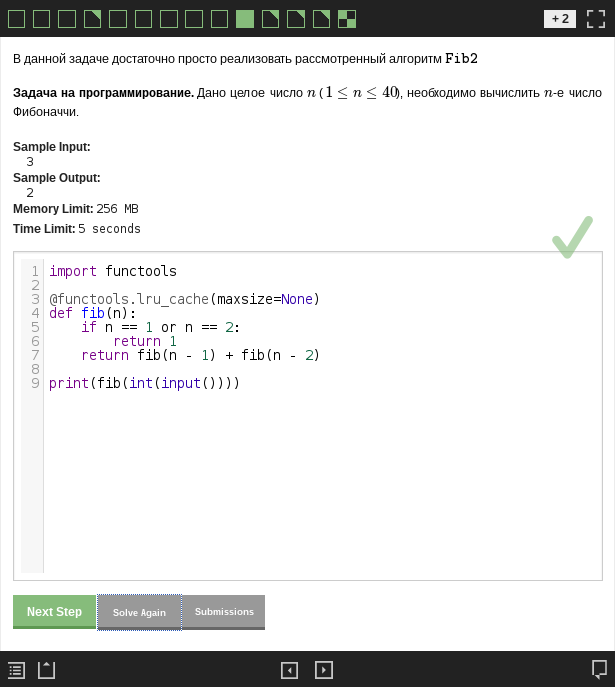
\includegraphics[width=\textwidth]{../res/quiz.png}
      \caption{Пример упражнения (code)}
      \label{fig:1}
    \end{figure}
  \end{columns}
\end{frame}

\begin{frame}{API}
  \begin{columns}[t]
    \column{.5\textwidth}
    Сервер
    \begin{itemize}
    \item Python
    \item JSON (eDSL для описания схем)
    \item асинхронность
    \end{itemize}

    \column{.5\textwidth}
    Клиент
    \begin{itemize}
    \item Handlebars
    \item JavaScript / простые функции
    \item CoffeScript / Ember компоненты
    \end{itemize}
  \end{columns}

  \bigskip

  Сервер для тестирования/разработки.

  \medskip

  Модуль упражнения от стороннего разработчика!
\end{frame}

\begin{frame}{Изоляция и масштабирование}
  \begin{itemize}
  \item Расширение codejail(мультиязычность, сообщения об ошибках,
    коммуникация...)
  \item Создание профилей apparmor.
  \item Масштабируемость при помощи celry.
  \item TODO: управление конфигурациями.
  \end{itemize}
\end{frame}

\begin{frame}{Результаты}
  \begin{itemize}
  \item[\checkmark] Реализовано 9 типов упражнений, которые успешно использованы
    в крупных курсах.
  \item[\checkmark] Разработано API для создания новых типов упражнений. С его
    помощью сторонним разработчиком создан новый тип упражнения.
  \item[\checkmark] На основе celery и codejail создана система масштабируемого и
    безопасного исполнения кода.
  \end{itemize}
\end{frame}

\end{document}